\chapter{PHÂN TÍCH VÀ THIẾT KẾ HỆ THỐNG}\label{chap2_intro}
\vspace{-40pt}

\section{Yêu cầu hệ thống}
\subsection{Yêu cầu chức năng}
\begin{functionalrequirementtable}
    \textbf{UC01 --} & \textbf{Đăng ký:} & Người dùng chưa đăng nhập có thể tạo tài khoản mới; hệ thống kiểm tra tính đầy đủ, hợp lệ của thông tin trước khi lưu. \\ \hline
    \textbf{UC02 --} & \textbf{Đăng nhập:} & Người dùng cung cấp thông tin xác thực; hệ thống kiểm tra thông tin đăng nhập và trạng thái tài khoản trước khi cho phép truy cập. \\ \hline
    \textbf{UC03 --} & \textbf{Xem, tìm kiếm và lọc sản phẩm:} & Người dùng có thể xem sản phẩm, tìm kiếm theo từ khóa, lọc theo danh mục, khoảng giá hoặc thương hiệu và xem thông tin chi tiết. \\ \hline
    \textbf{UC04 --} & \textbf{Quản lý giỏ hàng:} & Khách hàng có thể thêm sản phẩm vào giỏ hàng, thay đổi số lượng hoặc xóa sản phẩm; giỏ hàng được quản lý theo tài khoản. \\ \hline
    \textbf{UC05 --} & \textbf{Đặt hàng:} & Khách hàng tạo đơn từ giỏ hàng, chọn địa chỉ nhận hàng, có thể áp dụng voucher và chọn phương thức thanh toán; hệ thống kiểm tra thông tin, ưu đãi và tồn kho trước khi tạo đơn. \\ \hline
    \textbf{UC06 --} & \textbf{Thanh toán:} & Khách hàng thanh toán khi nhận hàng hoặc trực tuyến; với giao dịch trực tuyến, hệ thống gửi yêu cầu đến cổng thanh toán và cập nhật trạng thái theo kết quả. \\ \hline
    \textbf{UC07 --} & \textbf{Theo dõi và hủy đơn hàng:} & Khách hàng xem đơn hàng, theo dõi trạng thái xử lý và thanh toán, đồng thời gửi yêu cầu hủy khi đơn còn ở trạng thái cho phép. \\ \hline
    \textbf{UC08 --} & \textbf{Quản lý tài khoản:} & Khách hàng xem và cập nhật thông tin cá nhân, thông tin liên hệ, mật khẩu và sổ địa chỉ giao hàng. \\ \hline
    \textbf{UC09 --} & \textbf{Quản lý đơn hàng:} & Nhân viên và quản trị viên xem, kiểm tra và xử lý đơn hàng theo quyền được cấp, từ xác nhận đơn đến cập nhật trạng thái xử lý. \\ \hline
    \textbf{UC10 --} & \textbf{Kiểm tra tồn kho:} & Nhân viên tra cứu số lượng tồn kho của sản phẩm; chức năng này chỉ phục vụ xem thông tin, không điều chỉnh số lượng. \\ \hline
    \textbf{UC11 --} & \textbf{Quản lý sản phẩm:} & Quản trị viên thêm, chỉnh sửa và cập nhật trạng thái sản phẩm, bao gồm thông tin mô tả, giá niêm yết, phân loại và thông số kỹ thuật. \\ \hline
    \textbf{UC12 --} & \textbf{Quản lý danh mục:} & Quản trị viên thêm, chỉnh sửa hoặc cập nhật trạng thái danh mục sản phẩm. \\ \hline
    \textbf{UC13 --} & \textbf{Quản lý người dùng:} & Quản trị viên tìm kiếm và quản lý tài khoản; có thể thêm hoặc cập nhật tài khoản nhân viên, cũng như xem và thay đổi trạng thái tài khoản khách hàng. \\ \hline
    \textbf{UC14 --} & \textbf{Quản lý kho:} & Quản trị viên theo dõi tồn kho và nhập hoặc điều chỉnh số lượng sản phẩm; hệ thống kiểm tra dữ liệu để số lượng không nhỏ hơn 0. \\ \hline
    \textbf{UC15 --} & \textbf{Xem thống kê:} & Quản trị viên xem số liệu về doanh thu, đơn hàng và tình hình sản phẩm theo khoảng thời gian được chọn. \\ \hline
    \textbf{UC16 --} & \textbf{Quản lý chương trình giảm giá:} & Quản trị viên tạo, chỉnh sửa, kích hoạt hoặc kết thúc chương trình giảm giá, áp dụng cho toàn trang hoặc sản phẩm được chọn với mức giảm theo phần trăm hoặc số tiền. \\ \hline
    \textbf{UC17 --} & \textbf{Quản lý voucher:} & Quản trị viên tạo và quản lý voucher, gồm mã, mức giảm, thời hạn, giá trị đơn tối thiểu và các giới hạn sử dụng. \\ \hline
    \textbf{UC18 --} & \textbf{Áp dụng voucher khi đặt hàng:} & Khách hàng nhập mã voucher khi đặt hàng; hệ thống kiểm tra điều kiện và giới hạn sử dụng, tính lại tổng tiền và ghi nhận lượt sử dụng khi tạo đơn. \\ \hline
\end{functionalrequirementtable}

\subsection{Yêu cầu phi chức năng}
Thông tin đầu vào cần được kiểm tra trước khi xử lý; thao tác thay đổi dữ liệu cần được thực hiện qua các luồng có kiểm soát. Dữ liệu tài khoản và đơn hàng được lưu trong cơ sở dữ liệu MySQL. Giao diện cần trình bày các chức năng rõ ràng trên trình duyệt máy tính và có thể sử dụng các tương tác JavaScript hiện có.

\section{Tác nhân và quy tắc nghiệp vụ}
\subsection{Tác nhân}
\begin{usecasetable}
    \textbf{Khách vãng lai:} & Là người truy cập website nhưng chưa được xác thực đăng nhập vào hệ thống. Khách vãng lai có thể đã có hoặc chưa có tài khoản. Tác nhân này chỉ có quyền đăng ký, đăng nhập, xem, tìm kiếm và lọc sản phẩm. Nếu muốn thực hiện thao tác với giỏ hàng hoặc mua hàng, hệ thống sẽ yêu cầu Khách vãng lai phải đăng nhập để chuyển thành Khách hàng. \\ \hline
    \textbf{Khách hàng:} & Là người đã có tài khoản và đăng nhập vào hệ thống. Khách hàng có thể xem sản phẩm, quản lý giỏ hàng, đặt hàng, thanh toán, theo dõi và hủy đơn hàng theo điều kiện cho phép, đồng thời quản lý thông tin tài khoản \\ \hline
    \textbf{Nhân viên:} & Hỗ trợ hoạt động bán hàng và xử lý đơn hàng trong phạm vi quyền được cấp và chỉ có thể kiểm trasố lượng tồn kho của sản phẩm. \\ \hline
    \textbf{Quản trị viên:} & Là người có quyền quản lý và vận hành hệ thống. Quản trị viên có thể quản lý đơn hàng, sản phẩm, danh mục, người dùng, kho và xem các số liệu thống kê. \\ \hline
    \textbf{Cổng thanh toán:} & Là hệ thống thanh toán bên ngoài được sử dụng để xử lý các giao dịch thanh toán trực tuyến và trả kết quả giao dịch về cho hệ thống. \\ \hline
    \textbf{Google Identity:} & Là dịch vụ xác thực của Google cho phép người dùng đăng nhập vào hệ thống bằng tài khoản Google của họ. \\ \hline
\end{usecasetable}

\subsection{Quy trình xử lý đơn hàng}

Quy trình xử lý đơn hàng trong hệ thống được xác định như sau:

\begin{center}
Chờ xác nhận $\rightarrow$ Đang chuẩn bị hàng $\rightarrow$ Đang giao hàng $\rightarrow$ Hoàn thành / Giao hàng thất bại
\end{center}

Ngoài luồng xử lý chính, đơn hàng có thể chuyển từ trạng thái \textbf{Chờ xác nhận} sang \textbf{Đã hủy} khi khách hàng thực hiện hủy đơn theo điều kiện cho phép, hoặc hệ thống tự động hủy do thanh toán không thành công hoặc quá thời gian thanh toán quy định.

\subsection{Quy tắc chuyển trạng thái đơn hàng}

\begin{itemize}
\item \textbf{Chờ xác nhận $\rightarrow$ Đang chuẩn bị hàng:} Nhân viên hoặc Quản trị viên xác nhận đơn hàng sau khi kiểm tra thông tin hợp lệ.

\item \textbf{Chờ xác nhận $\rightarrow$ Đã hủy:} Khách hàng được phép hủy đơn khi đơn hàng chưa được xác nhận; hệ thống tự động hủy đơn khi giao dịch thanh toán không thành công hoặc quá thời gian thanh toán quy định.

\item \textbf{Đang chuẩn bị hàng $\rightarrow$ Đang giao hàng:} Đơn hàng đã được chuẩn bị và chuyển sang quá trình giao hàng.

\item \textbf{Đang giao hàng $\rightarrow$ Hoàn thành:} Đơn hàng hoàn tất quá trình giao hàng thành công.

\item \textbf{Đang giao hàng $\rightarrow$ Giao hàng thất bại:} Giao hàng không thành công, chẳng hạn khách hàng từ chối nhận hàng hoặc shipper không thể liên lạc; đơn hàng được xử lý hoàn về kho.

\item Không cho phép chuyển trạng thái tùy ý; trạng thái mới phải phù hợp với quy trình xử lý đơn hàng.

\item Đơn hàng đã ở trạng thái \textbf{Đã hủy}, \textbf{Giao hàng thất bại} hoặc \textbf{Hoàn thành} không được chuyển sang trạng thái xử lý khác.
\end{itemize}
\subsection{Quy tắc hủy đơn hàng}
\begin{itemize}
    \item Khách hàng chỉ được phép hủy đơn khi đơn hàng đang ở trạng thái \textbf{Chờ xác nhận}.
    \item Khách hàng không được phép tự hủy đơn khi đơn hàng đang ở trạng thái \textbf{Đang chuẩn bị hàng}, \textbf{Đang giao hàng} hoặc \textbf{Hoàn thành}.
    \item Đơn hàng đã ở trạng thái \textbf{Đã hủy} không thể thực hiện thao tác hủy lại.
\end{itemize}

\subsection{Quy tắc quản lý tồn kho}

\begin{itemize}
\item Khi khách hàng đặt hàng thành công (tạo đơn hàng), hệ thống sẽ ngay lập tức \textbf{tạm trừ (giữ chỗ)} số lượng tồn kho của các sản phẩm tương ứng.
\item Không cho phép tạo đơn hàng nếu số lượng tồn kho hiện tại không đủ đáp ứng số lượng trong giỏ hàng.
\item Nếu đơn hàng chuyển sang trạng thái \textbf{Đã hủy} (do khách hàng hủy hoặc hệ thống tự động hủy do quá hạn thanh toán), hệ thống sẽ tự động \textbf{cộng trả lại} số lượng tồn kho đã tạm trừ.
\item Nếu đơn hàng chuyển sang trạng thái \textbf{Giao hàng thất bại}, hệ thống sẽ \textbf{cộng trả lại} số lượng tồn kho sau khi xác nhận hàng hoàn về kho.
\item Việc kiểm tra và tạm trừ tồn kho ngay tại thời điểm khách hàng đặt hàng giúp tránh tình trạng nhiều khách hàng cùng đặt một sản phẩm trong khi số lượng tồn kho có hạn.
\item Hệ thống không cho phép số lượng tồn kho nhỏ hơn 0.
\end{itemize}


\subsection{Quy tắc thanh toán}

Hệ thống hỗ trợ hai phương thức thanh toán cơ bản:

\begin{itemize}
    \item \textbf{Thanh toán khi nhận hàng (COD):} Khi đơn hàng được tạo, trạng thái thanh toán được ghi nhận là \textbf{Chưa thanh toán}. Khách hàng thực hiện thanh toán khi nhận hàng. Khi giao dịch COD được hoàn tất thành công, trạng thái thanh toán của đơn hàng được cập nhật thành \textbf{Đã thanh toán}.

    \item \textbf{Thanh toán trực tuyến:} Hệ thống gửi yêu cầu giao dịch đến Cổng thanh toán. Chỉ khi nhận được kết quả giao dịch hợp lệ và thành công, hệ thống mới cập nhật trạng thái thanh toán thành \textbf{Đã thanh toán}.
\end{itemize}

Trạng thái thanh toán gồm:

\begin{itemize}
    \item \textbf{Chưa thanh toán:} Đơn hàng chưa ghi nhận thanh toán thành công.
    \item \textbf{Đã thanh toán:} Đơn hàng đã ghi nhận thanh toán thành công.
\end{itemize}

\subsection{Quy tắc xử lý thanh toán trực tuyến thất bại}

\begin{itemize}
    \item Nếu giao dịch trực tuyến thất bại hoặc bị khách hàng hủy, hệ thống giữ trạng thái thanh toán là \textbf{Chưa thanh toán} và thông báo kết quả cho khách hàng.

    \item Đối với đơn hàng vẫn còn hiệu lực và đang ở trạng thái chưa thanh toán, khách hàng được phép thực hiện lại thao tác thanh toán trực tuyến.

    \item Hệ thống không tự động chuyển trạng thái thanh toán thành \textbf{Đã thanh toán} nếu chưa nhận được kết quả giao dịch thành công hợp lệ từ Cổng thanh toán.

    \item Đơn hàng đã ở trạng thái \textbf{Đã thanh toán} không được thực hiện thanh toán lại.

    \item Đơn hàng đã ở trạng thái \textbf{Đã hủy} không được thực hiện thanh toán.

    \item Việc chuyển đổi từ thanh toán trực tuyến sang COD chỉ được thực hiện nếu hệ thống có hỗ trợ chức năng thay đổi phương thức thanh toán.
\end{itemize}
\section{Thiết kế kiến trúc}
Hệ thống được tổ chức quanh front controller và router. Router chuyển yêu cầu đến controller tương ứng; controller gọi model để thực hiện nghiệp vụ và lấy dữ liệu; view nhận dữ liệu để hiển thị trang. Các model kết nối MySQL thông qua PDO. Cấu trúc này giữ phần giao diện tách biệt tương đối với xử lý nghiệp vụ và truy vấn dữ liệu.

\section{Thiết kế cơ sở dữ liệu}
Cơ sở dữ liệu lưu trữ các nhóm thông tin chính: người dùng và tài khoản; danh mục và sản phẩm; giỏ hàng và chi tiết giỏ hàng; đơn hàng và chi tiết đơn hàng; lịch sử kho. Các bảng được liên kết bằng khóa chính, khóa ngoại và các ràng buộc phù hợp với quan hệ nghiệp vụ. Bảng giao dịch thanh toán có trong schema nhưng chưa được sử dụng trong luồng đặt hàng hiện tại.

\section{Công cụ và môi trường}
Ứng dụng được xây dựng bằng PHP, MySQL, HTML, CSS và JavaScript; PDO được dùng để kết nối cơ sở dữ liệu. Môi trường triển khai của dự án sử dụng máy chủ web Apache trong bộ XAMPP.

\section{Sơ đồ Use Case tổng quan}
\begin{figure}[H]
    \centering
    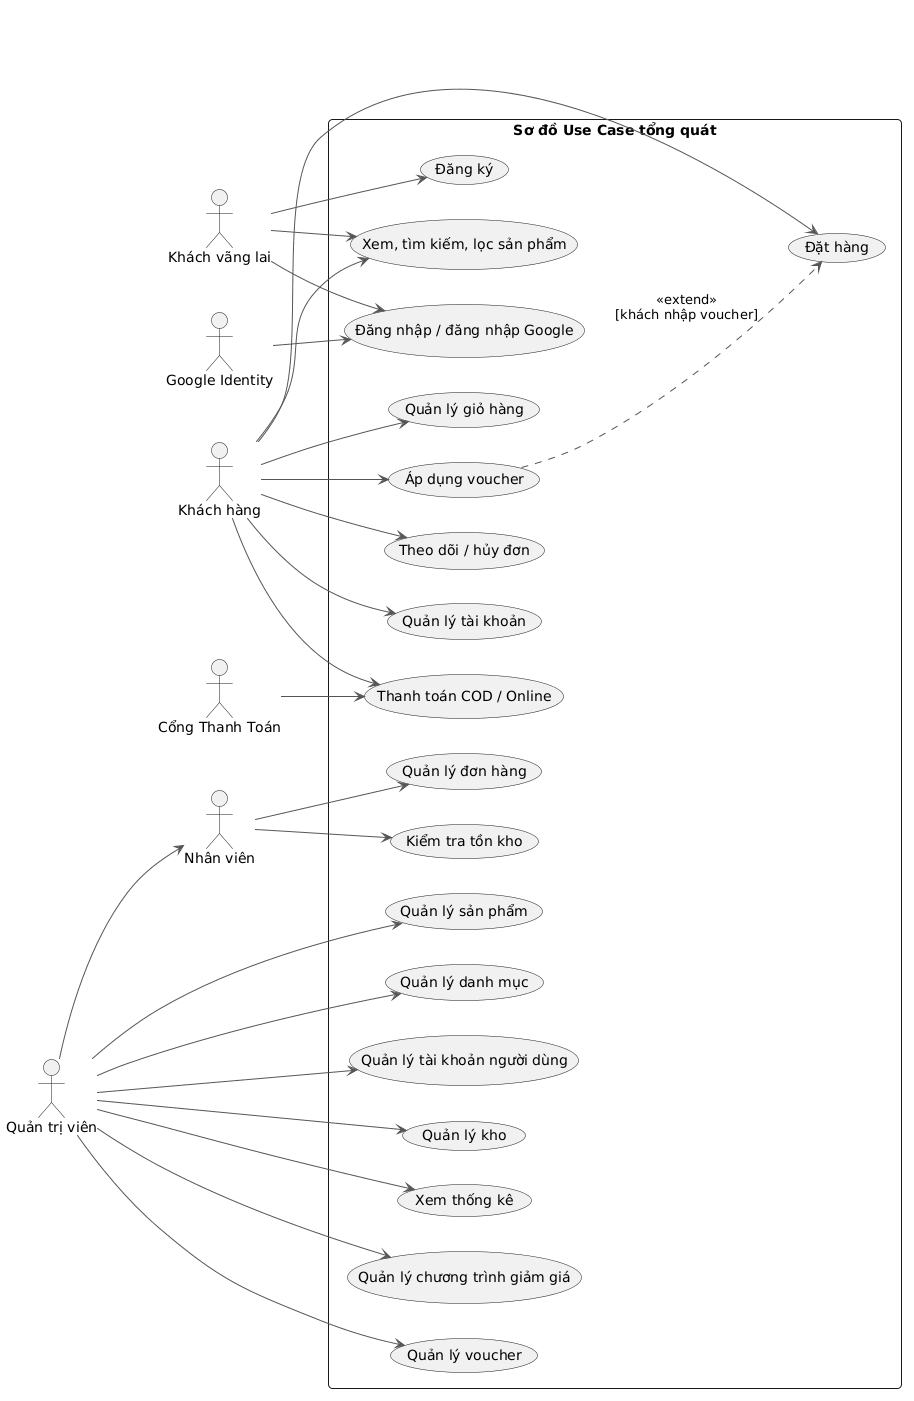
\includegraphics[width=0.72\textwidth, keepaspectratio]{Chapter_2/Images_c2/So_do_UC_tong_quan.png}
    \caption{Sơ đồ Use Case tổng quát của hệ thống website T\&T Computer}
    \label{fig:use-case-tong-quan}
\end{figure}

\section{Sơ đồ cơ sở dữ liệu:}
\begin{figure}[H]
    \centering
    \includegraphics[width=0.9\textwidth, keepaspectratio]{Chapter_2/images_c2/db.png}
    \caption{Sơ đồ cơ sở dữ liệu}
    \label{fig:db-diagram}
\end{figure}

\section{Sơ đồ lớp:}
\begin{figure}[H]
    \centering
    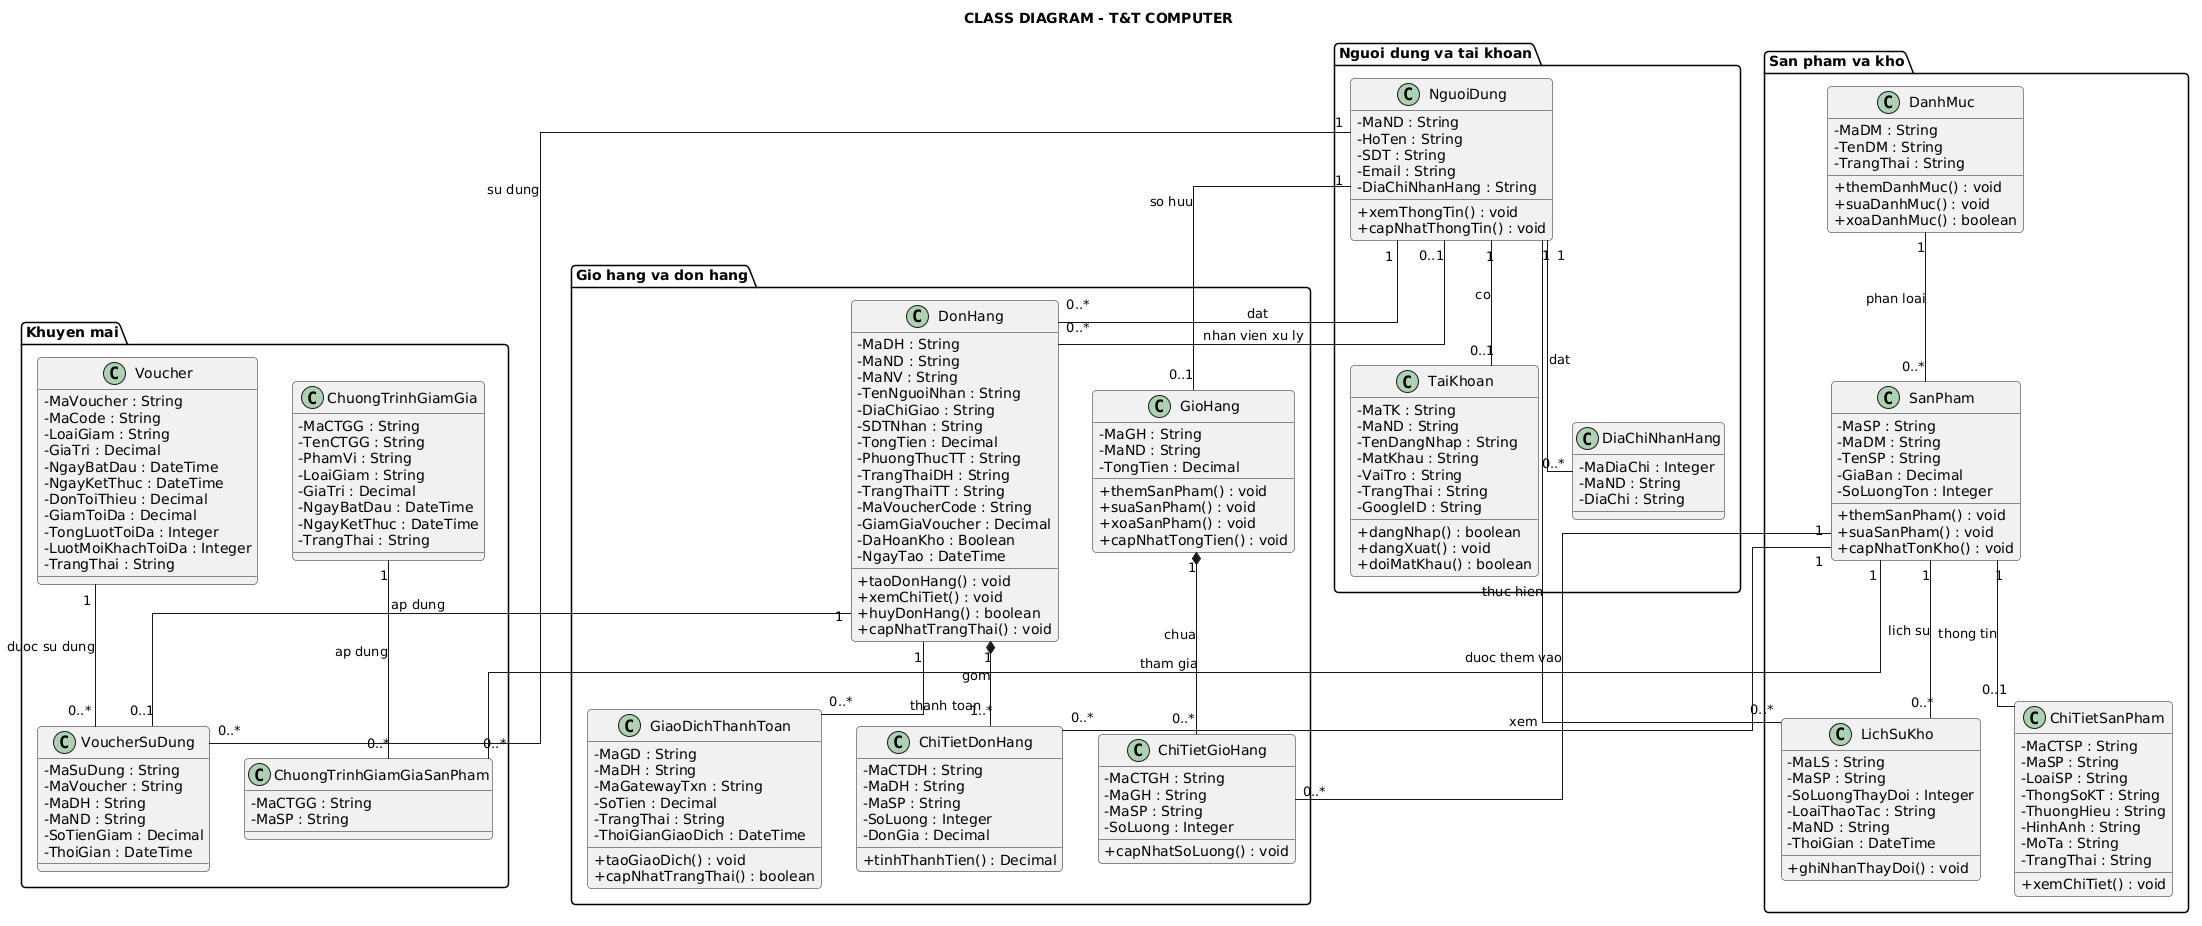
\includegraphics[width=0.9\textwidth, keepaspectratio]{Chapter_4/image/Sơ đồ class.png}
    \caption{Sơ đồ lớp}
    \label{fig:class-diagram}
\end{figure}
